\section{Referencial Teórico} \label{sec:refTeorico}
Nesta seção, serão abordados conceitos fundamentais para a compreensão dessa proposta, são eles: Inteligência Artificial, Internet das Coisas (IoT), Microcomputador, Servo Motor, Sensor Ultrassônico, Válvulas Selenóide e bombeamento de água. 

\subsection{Inteligência Artificial}
A inteligência artificial (IA), conforme definido pela \cite{ia}, já é parte da tecnologia moderna, pois, ela torna possível o aprendizado de máquina e a tomada de decisões, em uma velocidade e eficiência superiores aos seres humanos.

A IA desempenha um papel fundamental em diversos aspectos de nossa vida cotidiana, desde assistentes virtuais presentes em nossos smartphones até carros autônomos que podem navegar por conta própria. Pense em ter um amigo digital que compreende suas palavras, responde às suas perguntas e até mesmo antecipa suas necessidades futuras. A IA é essa amiga digital, e sua habilidade de aprender com a experiência a torna cada vez mais inteligente com o tempo.

À medida que a IA continua a evoluir nos apresenta novas formas de   tornar nossas vidas mais convenientes e eficazes. No entanto, também suscita questões cruciais relacionadas à privacidade e ética que exigem uma atenção cuidadosa. Em resumo, a inteligência artificial é uma tecnologia que está transformando nosso mundo de maneiras fascinantes e revolucionárias, tal como definiu \cite{John}, o pai da IA, como "a ciência e a engenharia de criar máquinas inteligentes".


\subsection{Internet das Coisas (IoT)}
A Internet das Coisas (IoT), conforme descrita pela \cite{iot}, representa uma revolução tecnológica que viabiliza a interconexão de objetos em nosso cotidiano, conferindo-lhes a capacidade de comunicação e coleta de dados. Em termos simples, trata-se da habilidade de dispositivos comuns, incluindo eletrodomésticos, sensores, veículos e até mesmo roupas, conectarem-se à internet e compartilharem informações entre si.
=90
Essa rede de objetos inteligentes tem a capacidade de coletar, analisar e compartilhar dados relevantes, contribuindo para aprimorar a eficiência, automação e comodidade nas atividades do dia a dia. Um exemplo prático é a capacidade de um termostato ajustar a temperatura da sua residência com base nas informações de previsão do tempo ou de uma pulseira que monitora sua saúde e envia dados ao seu médico. Em resumo, a IoT representa um avanço tecnológico que torna nossos objetos cotidianos mais inteligentes e interconectados, com o propósito de melhorar nossas vidas.

\subsection{Single Board Computer}Single Board Computer
Um microcomputador, como descrito no site oficial do \cite{raspberry}, é um tipo de computador pessoal notavelmente compacto, projetado para executar tarefas diversificadas e específicas. Estes dispositivos, frequentemente do tamanho de um cartão de crédito, ou ainda menores, são equipados com componentes de processamento, memória e conectividade que lhes permitem desempenhar uma ampla variedade de funções.

 Apesar de sem enquardar perfeitamente na definição de acima, o Raspberry Pi na verdade é um exemplo de SBC (Single Board Computer), que ganhou ampla popularidade. O SBC oferece capacidades de processamento, entrada/saída e conectividade, bem como a capacidade de executar sistemas operacionais, o que possibilita aos usuários a realização de diversas tarefas, desde programação e navegação na web até o controle de dispositivos eletrônicos.

A característica distintiva dos microcomputadores reside em sua portabilidade e versatilidade. Eles encontram aplicação em projetos de automação residencial, sistemas de monitoramento, servidores domésticos e muito mais. A acessibilidade e a facilidade de programação tornam os microcomputadores uma ferramenta valiosa tanto para entusiastas quanto para desenvolvedores e educadores interessados em explorar o campo da eletrônica e da computação.

Em resumo, um microcomputador é uma categoria de dispositivos eletrônicos compactos e versáteis, que oferece uma plataforma para experimentação, aprendizado e desenvolvimento de projetos em diversas áreas, desde eletrônica até automação e computação.

\subsubsection{Raspberry Pi}
 A Figura 1 apresenta o Raspberry Pi, conforme explicado no site oficial do \cite{raspberry}, é um SBC de placa única pois todos os principais componentes de um computador, como processador, memória e conectividade, estão integrados em uma única placa, proporcionando funcionalidade completa em um espaço compacto, ao qual se destaca pela sua versatilidade e facilidade de uso. Embora seja do tamanho de um cartão de crédito, este dispositivo é equipado com recursos de processamento e conectividade que o tornam incrivelmente versátil.

O Raspberry Pi é um sistema completo, com portas USB para conexão de teclado, mouse e outros dispositivos, bem como portas HDMI para conexão a um monitor ou TV. Além disso, ele possui portas GPIO (Entrada/Saída de Propósito Geral) que possibilitam a interação com sensores, LEDs e outros dispositivos eletrônicos.

O Raspberry Pi é capaz de executar sistemas operacionais, como o Raspberry Pi OS, que podem ser instalados em um cartão microSD. Isso possibilita a execução de uma ampla variedade de aplicativos e a realização de tarefas, como navegação na web, programação, reprodução de mídia e até mesmo a criação de servidores.

Este SBC é frequentemente utilizado em projetos de automação residencial, robótica, educação em programação, servidores domésticos e muito mais. Sua acessibilidade e recursos tornam o Raspberry Pi uma plataforma ideal para explorar a computação, eletrônica e desenvolvimento de projetos.

Ou seja, o Raspberry Pi é um SBC de baixo custo que oferece uma ampla gama de possibilidades para aprendizado e desenvolvimento de projetos, tornando-o uma ferramenta ideal para explorar o mundo da tecnologia de forma criativa e prática.

 \begin{figure}[H]
    \caption{Raspberry Pi}
    \label{fig:raspberryImagem}
    \begin{center}
        
        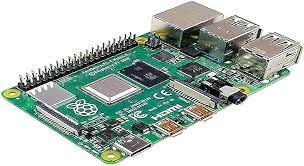
\includegraphics[scale=1]{Textuais/imagens/raspberry.png}
        
        Fonte:  Aliexpress
    \end{center}
\end{figure}

\subsection{Servo Motor}
Na Figura 2 temos um exemplo de servo motor, que é definido no site  \cite{servomotor} como um dispositivo eletromecânico projetado para controlar a posição de uma haste ou alavanca em resposta a um sinal de controle. Esse tipo de dispositivo é amplamente empregado em diversas aplicações que demandam movimentos precisos, como na área de robótica, sistemas de automação industrial e modelagem de aeromodelismo. O servo motor é reconhecido por sua habilidade em girar ou mover-se até uma posição específica, obedecendo comandos precisos, tornando-o uma escolha proeminente para o controle de movimentos de alta precisão.

O funcionamento do servo motor é fundamentado em um sistema interno de feedback. Ele consiste de um motor elétrico, um conjunto de engrenagens e, normalmente, um dispositivo de feedback, que frequentemente é um potenciômetro. Quando um sinal de controle é aplicado ao servo motor, o motor se movimenta com o intuito de posicionar a haste ou alavanca na direção desejada. O dispositivo de feedback mantém constante monitoramento da posição atual e transmite informações ao controlador do servo motor, permitindo-lhe realizar ajustes precisos para manter a posição desejada.

A capacidade intrínseca de controle preciso faz do servo motor a escolha ideal para aplicações que requerem movimentos angulares específicos, como o ajuste da posição de um braço robótico ou a direção das rodas de um veículo autônomo. Além disso, os servo motores são extensivamente aplicados na área de aeromodelismo, onde controlam superfícies como lemes e ailerons.

Resumindo, o servo motor é um dispositivo eletromecânico projetado para efetuar um controle preciso da posição de uma haste ou alavanca em resposta a comandos. Essa característica o torna fundamental em diversas aplicações que exigem movimentos controlados e precisos.

 \begin{figure}[H]
    \caption{Servo Motor}
    \label{fig:servomotorImagem}
    \begin{center}
        
        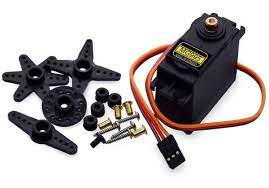
\includegraphics[scale=1]{Textuais/imagens/servomotor.png}
        
        Fonte: Mercado Livre
    \end{center}
\end{figure}

\subsection{Válvula Solenoide}
Uma válvula solenoide, conforme detalhado no manual de instalação de válvulas solenoide da \cite{valvula} e apresentado na Figura 3, é um dispositivo eletromecânico projetado para regular o fluxo de fluidos, como líquidos ou gases, em sistemas de tubulação. A operação desse dispositivo é baseada nos princípios da eletricidade e do magnetismo. A componente essencial da válvula solenoide é uma bobina eletromagnética que, quando alimentada eletricamente, cria um campo magnético. Esse campo magnético age sobre uma haste móvel, conhecida como núcleo, localizada no interior da bobina. Quando o núcleo é atraído pelo campo magnético, ele movimenta um obturador ou diafragma, resultando na abertura ou fechamento da passagem do fluido através da válvula.

As válvulas solenoides encontram uma ampla gama de aplicações, abrangendo desde sistemas de irrigação e controle de fluidos industriais até eletrodomésticos, como máquinas de lavar e cafeteiras. Elas proporcionam uma forma eficaz e precisa de gerenciar o fluxo de fluidos, sendo ativadas por meio de sinais elétricos. Isso permite que as válvulas solenoides sejam controladas remotamente e automatizadas conforme as exigências do sistema.

Resumidamente, uma válvula solenoide é um dispositivo eletromecânico que regula o fluxo de líquidos ou gases em sistemas, realizando tal controle por meio da ativação de uma bobina eletromagnética. Sua versatilidade e precisão a tornam uma solução comum em uma variedade de aplicações, assegurando um controle eficiente e confiável de fluidos em diversos sistemas.

 \begin{figure}[H]
    \caption{Válvula Selenóide}
    \label{fig:valvulaImagem}
    \begin{center}
        
        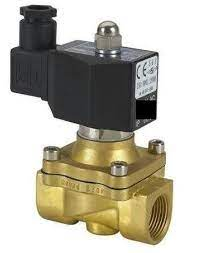
\includegraphics[scale=1]{Textuais/imagens/valvula.png}
        
        Fonte: Amazon
    \end{center}
\end{figure}

\subsection{Bombeamento de água}
Sistema de Bombeamento de Água: O sistema de bombeamento de água, conforme detalhado no site da \cite{bomba}, a mini bomba de agua 12V RS385 foi projetada com foco na prototipagem e é especialmente adequada para aplicações em automação residencial (domótica) e protótipos de robótica baseados em microcontroladores populares, como Arduino e Raspberry Pi. Figura 4 é um exemplo de bomba de água.

Com seu motor de tamanho apropriado, esta bomba é capaz de impulsionar uma quantidade de água significativa, variando de 1500ml a 2000ml por minuto. Sua eficiência e precisão se destacam, particularmente quando utilizada em conjunto com dispositivos como o Arduino.

Esta bomba encontra aplicação em uma variedade de projetos, incluindo carrinhos ou robôs de combate a incêndios, robôs hidráulicos e sistemas de irrigação automática, com foco na automação residencial. Sua versatilidade permite que sua criatividade determine sua aplicação final.

\begin{figure}[H]
    \caption{Bomba de água}
    \label{fig:bombaImagem}
    \begin{center}
        
        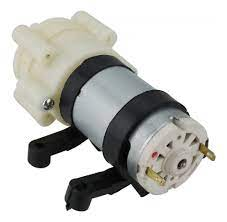
\includegraphics[scale=1]{Textuais/imagens/bomba.png}
        
        Fonte: Mercadolivre
    \end{center}
\end{figure}

\subsection{Sensor Ultrassônico HC-SR04} O sensor ultrassônico HC-SR04, descrito no \cite{sensor} e apresentado na Figura 5, é um dispositivo que utiliza ondas sonoras de alta frequência para medir distâncias. Funciona emitindo um sinal sonoro inaudível e, em seguida, registrando o tempo que leva para esse sinal retornar após refletir em um objeto. Com base nesse tempo, o sensor calcula a distância entre ele e o objeto com notável precisão. Este sensor é frequentemente utilizado em projetos que envolvem detecção de obstáculos, medição de níveis de líquidos e até mesmo a criação de sistemas de estacionamento automatizado. É uma ferramenta valiosa para tornar dispositivos autônomos mais conscientes de seu ambiente, contribuindo para uma variedade de aplicações, desde robótica até automação residencial.

 \begin{figure}[H]
    \caption{Sensor Ultrassônico HC-SR04}
    \label{fig:sensorImagem}
    \begin{center}
        
        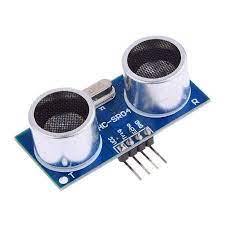
\includegraphics[scale=1]{Textuais/imagens/sensor.png}
        
        Fonte: Amazon
    \end{center}
\end{figure}
